% 来源：OEBPS/Text/Section0001_split_001.xhtml#sigil_toc_id_11

\BookChapter{3}
\section[第3章\q 利用复利魔力：做出一生最重要的财务决策]{第3章\\ 利用复利魔力：做出一生最重要的财务决策}

\begin{BookQuote}
我的财富来自三种要素的结合：生活在美国、一些幸运的基因、复利。

\hfill ——沃伦·巴菲特
\end{BookQuote}

我们现在开启投资自由之旅吧。利用复利的魔力，创造出真正巨大的财富。这并不是那种快速致富的计划，这也不是大多数人想的那种会让自己实现财务自由或者发财致富的计划。大多数人想的是“挣上一笔大钱”——发上一笔意外之财，然后他们觉得自己就会一直幸福地生活了。

但是我们还是面对现实吧，我们要谈的并不是“挣钱”致富。这是几百万名美国人重大的认识错误。我们误以为，只要自己工作更努力、更聪明、工作时间更长，就能实现自己的财务梦想。但只靠薪水，不管它有多高，都不能让你真正富有，实现财务自由。

我想起了这条真理，是在最近访问著名经济学家伯顿·麦基尔的时候，他写过一本金融行业的经典名著《漫步华尔街》。我专程前往普林斯顿大学拜访麦基尔教授，因为我不仅非常钦佩他的业绩，而且非常钦佩他直截了当的说话方式。不管是写作还是接受采访，他给人的印象都是直来直去的——我去见他那天也不例外。我想听听麦基尔教授的高见：在投资生涯的各个阶段，面临那些投资陷阱，人们应该如何应对呢？我想就我们可能面临的误区，听听他的见解。毕竟，麦基尔帮助投资界创立和发展了指数基金这个投资概念。指数基金能让一般投资者模拟整个市场进行投资；指数基金能让一般投资者，哪怕只有很少的资金，也能拥有整个股市的一部分，从而实现真正彻底的分散投资，而不必因为自己的财力和能力有限，只能购买一两只股票。如今，这类指数投资的资产规模超过7万亿美元！在我计划采访的很多投资大师中，麦基尔教授最有资格帮我拨开迷雾，看透证券市场那些投资机构的虚假广告宣传，戳穿那些投资机构故弄玄虚的专业术语，真实评估我们当前的投资环境。

我问麦基尔教授，大多数人刚开始投资会犯下的最大错误是什么。他没有丝毫犹豫，直截了当地告诉我：大多数人开始投资时，没有充分利用复利难以置信的巨大威力——复利能够利滚利，拥有翻倍再翻倍的增长魔力。

复利是力量无比强大的工具，以至爱因斯坦称复利是人类历史上最重要的发明。但是我心里嘀咕，如果复利真的有那么巨大的威力，那么为什么充分利用复利威力的人那么少呢？为了描述复利指数增长的威力，麦基尔教授和我分享了孪生兄弟威廉和詹姆斯的故事。他们两个人的投资策略简直是天壤之别。麦基尔教授在自己的书里讲过这个例子，所以我很熟悉。但听他亲口讲述，感觉非常美妙，有点儿像听81岁的布鲁斯·斯普林斯汀在自家客厅里表演有声版的《天生就会跑》一样。这个故事讲的是，孪生兄弟哥哥威廉和弟弟詹姆斯刚刚年满65岁，刚好到达男士传统的退休年龄。威廉投资起步比弟弟早，20岁的时候就开立了退休金账户，接下来20年里每年投资4000美元。到40岁的时候，他就不再往退休金账户里投钱了，而是把钱放在免税的投资领域，以获得每年10\%的税后净收益。

弟弟詹姆斯一直到40岁才开始储蓄养老金，而他哥哥这时已经停止储蓄了。像他哥哥一样，詹姆斯每年投资4000美元，每年也能获得10\%的收益，而且免税。但他一直这样投资持续到65岁——整整25年。

总的来说，哥哥威廉投资起步早，一共投入8万美元（4000美元/年×20年，每年投资收益率为10\%）。而弟弟詹姆斯投资起步晚，一共投入10万美元（4000美元/年×25年，每年投资收益率为10\%）。

那么到65岁退休的时候，兄弟俩谁的账户里的钱更多呢？

我知道麦基尔所讲的这个故事的结局，但他讲故事时充满愉悦和激情，好像第一次给别人讲这个故事一样。答案当然是起步早但投入少的那位哥哥威廉积累的钱更多。他比起步晚且投入更多的弟弟詹姆斯多赚多少钱呢？多了600\%。

现在让我们暂时回到过去，把这些数据放在历史环境中考虑一下。如果你是千禧一代或者是婴儿潮时代出生的人，一定要仔细看看下面这段话。你会知道，这个投资建议对你非常适用，不管你现在处于人生的哪个阶段，它都非常适用。如果你现在已经35岁了，突然明白了复利的巨大威力，你会觉得自己要是能早十年，25岁时就开始不断储蓄和投资利用复利来积累财富，那该有多好啊；如果你现在45岁，那你会非常希望自己能在35岁时就开始这样做了；如果你现在60多岁或者70多岁，你会想，如果自己能在十年前50多岁或者60多岁时就开始这样做，不断储蓄和投资利用复利来积累财富，那么自己可以积累起多么大一笔财富啊。如此类推，越早开始越好。

在麦基尔所举的例子中，两个孪生兄弟威廉和詹姆斯，哥哥威廉开始为养老储蓄投资的时间比较早，尽管在他弟弟开始储蓄投资之前他就停止追加投入了，但还是最终赚到了接近250万美元。而他的弟弟詹姆斯尽管一直储蓄且不断投入资金连续25年，直到65岁退休时总共积累的财富还不到45万美元。兄弟二人65岁时同时退休，但财富差距超过了200万美元！这都是因为威廉开始投资的时间早，充分利用了复利的巨大威力，使财富多增值了20年，结果给自己带来了无比巨大的领先优势。这样积累的巨大财富，让威廉的后半生衣食无忧，过上了相当富有的生活。

\begin{BookQuote}
山顶上的人不是从天上落到山顶上的。

\hfill ——文斯·隆巴迪
\end{BookQuote}

你是不是还不太相信，复利，长期而言，是唯一效果确定的方法呢？它能够让你的种子资金通过投资金融证券不断增值，让你最终获得丰厚收入，积累起巨大财富，足以满足你未来的需要。麦基尔分享了另外一个他非常喜欢的故事，从中你可以深刻领会他的观点。这个故事来自美国的历史教科书。当本杰明·富兰克林在1790年去世的时候，他分别留给波士顿和费城1000美元。他的馈赠附带了一些条件，具体而言，这些钱必须用来投资，而且未来100年都不能动。100年后，每个城市从账户中取出50万美元，用于指定的公共设施建设项目。账户剩余的钱在下个100年还是不能动，继续投资。最终，富兰克林去世后的200年里，美国股市的平均年复合收益率为8\%，每个城市都得到了其余的捐赠资金——1990年，接近650万美元。想象一下，1000美元竟然能够增值到650万美元，而且没有追加1美元的资金。

怎么会增加这么多钱呢？完全是复利的巨大力量！

是的，200年的时间确实很长。但3000\%的累计收益率，值得如此漫长的耐心等待。

麦基尔举的例子表明，我们内心早就认同了复利的力量：对于大多数人来说，我们现在的财富水平和我们想要的财富水平之间有着巨大的差距，只靠工作赚到的收入是永远无法填补的。因为只靠工作赚到的收入，永远无法比得上复利积累财富的巨大威力。

\begin{BookQuote}
如果只看经济方面的理由，有钱要比贫穷好。

\hfill ——伍迪·艾伦
\end{BookQuote}

你还是认为自己只靠工作赚钱就能实现财务自由吗？我们来快速浏览一些案例，看看那些世界上工作收入最高的人能不能最终实现财务自由。

传奇棒球投手科特·席林的职业生涯神奇得简直不可思议，帮助波士顿红袜队夺得了两个世界大赛总冠军，自己挣到了1亿美元。但是后来，他把自己所有的积蓄都投入了一家网络游戏创业企业，结果企业破产了——席林也破产了。“我从来不相信有人能击败我。”席林接受娱乐体育节目电视网的采访时说，“但我创业确实输了。”

过去赚到1亿美元的席林，现在负债5000万美元。

金·贝辛格是她那一代最受欢迎的女演员之一，在电影《爱你九周半》《蝙蝠侠》和《洛城机密》等热门影片中所扮演的角色令人难忘，因此获得奥斯卡金像奖最佳女配角奖，成为闪耀大银幕的超级巨星。作为最受欢迎的女演员之一，在事业的巅峰期，贝辛格平均每部电影的片酬高达1000万美元——她拍两部电影就能赚上2000万美元，这足够她在佐治亚州买下整整一座小镇了。

贝辛格最终却破产了。

马文·盖伊、威利·纳尔逊、M.C.哈默、密特·劳弗，这些歌星的专辑卖出了几百万张，开个演唱会就能让体育馆挤满歌迷。弗朗西斯·福特·科波拉导演了美国最伟大的电影之一《教父》，他能让影院爆满，至少在一段时间内确实如此，并创下了1.29亿美元的历史最高票房纪录。

但是这些巨星都曾濒临破产——科波拉大导演曾三次濒临破产。

“流行音乐天王”迈克尔·杰克逊，据报道曾签署一份价值近10亿美元的唱片合约，唱片销量超过7.5亿张。尽管如此，迈克尔·杰克逊2007年濒临破产，因为无法偿还梦幻庄园2500万美元的贷款。杰克逊花钱就像他永远也花不完一样，但是后来他还是花完了。两年后，杰克逊去世。据报道，他负债超过3亿美元。

你觉得，这些巨星会认为有一天自己的钱会停止流入吗？你认为，他们有没有考虑过为这一天做好准备呢？

你有没有注意到，不管你的工作能挣多少钱，你总有办法把它全部花掉？看看上面的例子，你可以清楚地看到，不只普通人，那些巨星也是如此。我们似乎都有方法挣多少就花多少，我想，有些人肯定花的比挣的还要多。我们经常看到，正是因为这个原因，很多超级巨星，尽管赚的特别多，但后来都一落千丈，穷到要破产——就像有些职业拳击手，靠比赛赢的钱比自己做梦梦到的还要多，可是后来花了个精光，还欠了一屁股债，在财务上输得如同在拳击台上被重重击倒。最典型的例子是，前世界重量级冠军迈克·泰森从富到穷再到破产的经历，他打拳赚到的钱超过历史上任何一位拳击手——接近5亿美元，后来却破产了。但是得到5个级别世界拳王金腰带的弗洛伊德·小梅威瑟，将要打破泰森的拳击收入纪录。跟泰森一样，小梅威瑟也是从一无所有的贫困生活中，一路“打”出来的。2013年9月，小梅威瑟在与卡内洛·阿瓦雷兹的比赛中获胜，稳赚4150万美元。由于电视转播按照收视次数计费，这让他的收入分成增加到8000多万美元，创下了历史纪录。这还只是他一场比赛的收入！在一天获得如此巨额收入之前，他已经进入《体育画报》美国最赚钱的运动员“财富50强”的名单。我个人非常喜欢小梅威瑟。他是个非常有天赋的运动员——目前少数非常有职业道德的运动员之一。他对自己的朋友极为慷慨。这个人身上有很多令人欣赏的优点。然而，小梅威瑟经过一路辛苦打拼，终于荣登美国最赚钱的运动员“财富50强”的榜首，却因为自己疯狂购物、毫无节制和胡乱投资，结果失去了所有财富。据报道，小梅威瑟花钱非常随意，最典型的例子是，他随身携带一个背包，里面装满了100万美元的现金——只是为了让自己随时能到路易·威登专卖店购买最时尚的服饰。

像许多成功人士一样，这些体育冠军也是绝顶聪明的家伙，我希望小梅威瑟现在能够走上投资正路，但根据小梅威瑟以前的商业合作伙伴，而且绝对可以说是赚钱的权威人士“50美分”（美国说唱歌手、企业家、投资商）所说的，这位拳击冠军除了拳击以外根本没有其他收入。这个说唱巨星用浅显易懂的几句话总结出了拳击选手的投资赚钱之道：“拳击，挣钱，花钱，拳击。拳击，挣钱，花钱，拳击。”

听起来这种理财方式很荒谬，不是吗？不幸的是，我们在某种程度上也与此没有差别。工作，挣钱，花钱，工作——这就是美国人最典型的理财方式！

\begin{BookQuote}
先听再说。写之前，先想。花钱之前，先赚。投资之前，先调查。批评之前，先等等。祈祷之前，先原谅。放弃之前，先试试。退休之前，先储蓄。临死之前，先赠予。

\hfill ——威廉·阿瑟·沃德
\end{BookQuote}

这是关系4150万美元的大问题：如果既有才华又有好运的超级巨星，通过工作赚到那么多钱都不能实现财务自由，你又怎么能期望通过工作赚钱来实现财务自由呢？

你肯定不能！

但你能做到的是，简单地改变一下你的投资理财策略，接受一个全新的思维模式。你必须掌控并利用复利让财富指数化增长的神奇力量。复利的力量会完全改变你的人生！你必须从给钱当仆人的层次，提升到让钱给你当仆人的更高层次。

现在是时候了，离开看台，进入赛场，加入比赛吧。因为最终想要实现财务自由，我们都必须成为投资者。

如果你已经是金融交易员了，你可能不会这样想，但如果你是为了生活、为了吃饭而工作，那你就是用时间换钱，甚至可以说是拿命换钱。坦率地说，这其实是你能做的最糟糕的交易。为什么？因为你总是能得到更多的钱，但你怎么也不可能得到更多的时间。

我不想讲得就像那些赚人眼泪的广告一样，但我们都知道生命无价，其实生命就是由很多分分秒秒构成的。你如果拿时间换钱，就会错过生命中的那些时时刻刻，就是拿命换钱。

当然，我们有时不得不错过一场舞蹈排练，或者错过一次晚上的约会，没办法，因为工作是你必须承担的责任，但我们需要经历那些时刻才能得到珍贵的记忆。这样的机会不是随时都有，想要就有的。

错过太多人生重要的时刻，你会开始怀疑，自己这样工作到底为了什么，这样做值得吗？

\subsection{终极自动取款机}

如果你需要钱，你去哪里取呢？你又不是世界冠军拳击手，背包里也没有装着100万厚厚的美元大钞，你需要什么样的自动取款机来取钱呢？

现在，我打赌，你生活中最主要的“赚钱机器”就是你自己。你可能也有一些投资，但是我敢说，你心里肯定没有把收入和这些投资联系到一起。你的工作停止了，你的赚钱机器就停止了，你的现金流就停止了，你的收入停止基本上意味着你的整个金融世界的运转就停止了，这是一个零和游戏，你放进去多少钱，意味着你能拿出来多少钱。

这样看来，你现在是另一种形式的自动取款机，只是对你个人而言，这是一笔“用时间换金钱”糟糕的交易，你实际上成了一个出卖时间的机器（更准确的表述是卖命的机器）。也许这听起来像科幻小说，但是对于大多数读者来说，这就是现实。你安排了这样的事情，让自己付出最宝贵的东西（时间），来换取你最需要的东西（金钱）。你如果聪明的话，一听就明白了，在用时间换金钱的这笔交易里，你是吃亏的那一方。

你听明白我说的意思了吧？你如果停止工作，就会停止赚钱，现在让我教你脱离这个财富方程式，然后寻找另一条积累财富的路径。我们来打造一个赚钱机器替代你，而且这样设计这个赚钱机器，让它能在你睡觉的时候照样不停地赚钱。你可以把这个赚钱机器想象成你创立的第二家企业，不用雇用员工，不用发工资，不用设立公司总部。这个企业唯一的库存就是你投入的钱。这家企业唯一的产品就是源源不断的收益，它永远不会干涸——即使你活到100岁。这家企业的使命就是给你和你的家庭提供终身的财务自由，或者给你未来的家庭，如果你现在还没有成家的话。

听起来是不是棒极了？你如果能打造出我说的这种神话般的机器，并合理地维护保养，那么它赚起钱来的威力就像1000台发电机同时发电一样巨大。这台赚钱的机器会像钟表一样不停地转动、不停地工作，一年365天都不休息；每到闰年它还会多工作一天，即使在国庆节（7月4日）那天也不例外。

看看下面这张图，你就会更加明白这台赚钱机器是怎样工作的。

\begin{figure}[htbp]
\centering
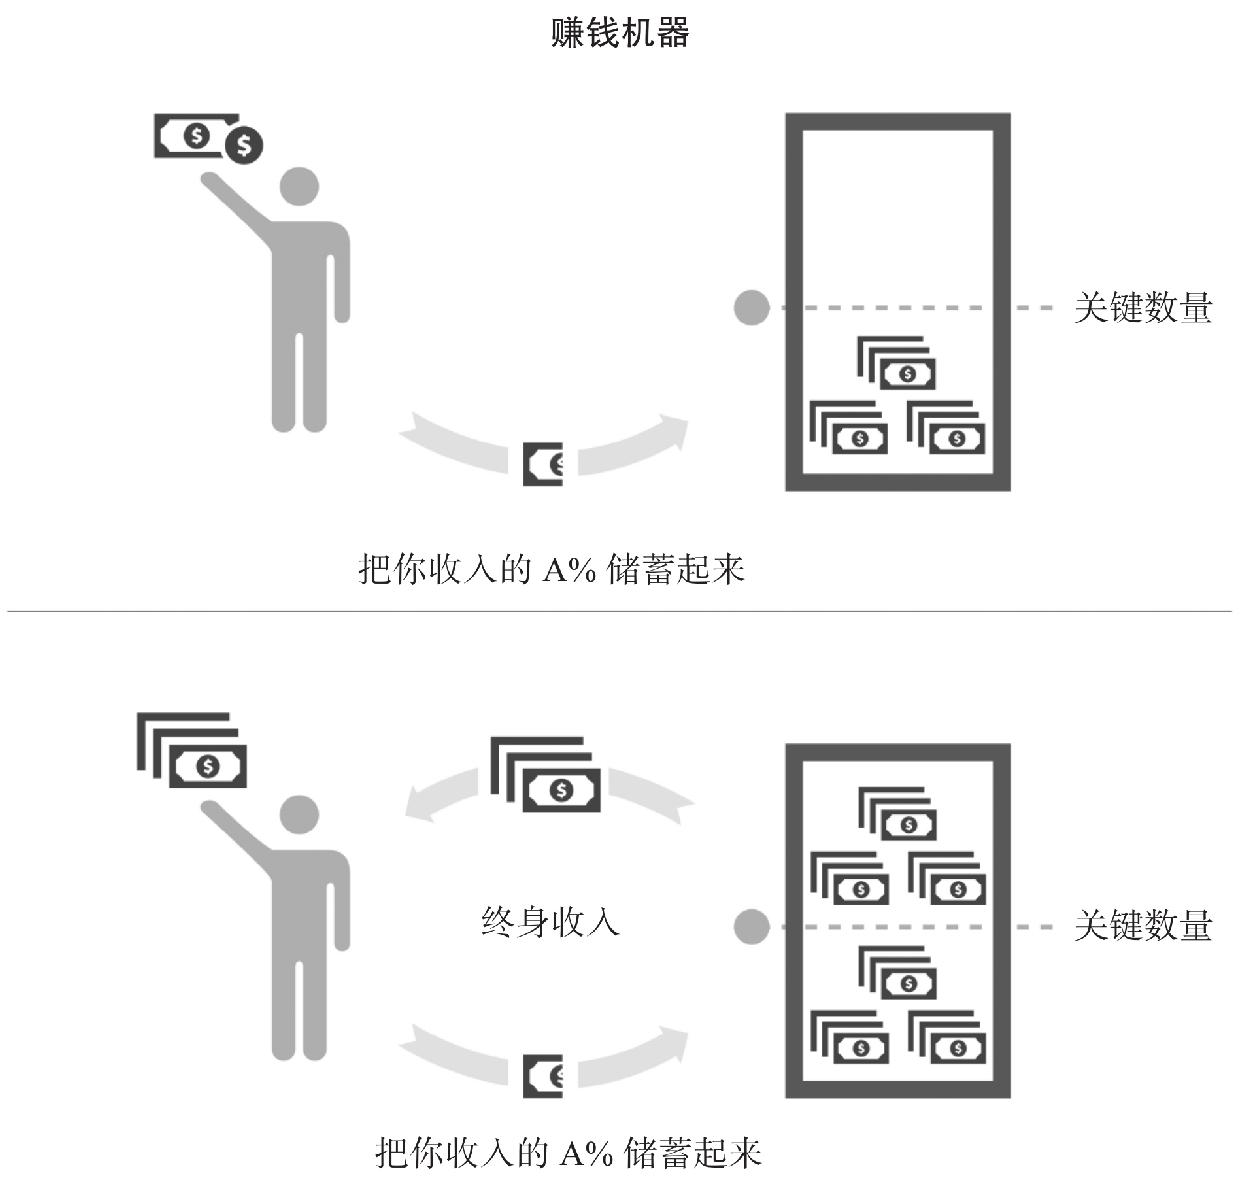
\includegraphics[width=0.70\linewidth,keepaspectratio]{image/3-1.jpg}
\caption{}\label{fig:3-1}
\end{figure}

你会看到，这台赚钱机器一直不动，直到你做出一生最重要的财务决策之后，它才会开始工作。什么财务决策如此重要呢？它就是你从工资收入里拿出来多少钱作为储蓄。也就是说，在你拿到工资收入之后，在支付自己的日常生活花费前，你先要决定从总收入中拿出来多大一部分付给自己。你能（更重要的是你愿意）从工资收入里拿出来多少钱储蓄起来，不管你生活是好是坏，这些钱你都不会动。我希望你一定要好好考虑这个用于储蓄的百分比，因为你的余生都取决于这个百分比。这样做的目标是让你能够告别朝九晚五的上班族生活，走上通向财务自由的道路。你开始这条财务自由之路的方法，就是做出一个简单的决策，开始利用复利的无与伦比的巨大力量。这个决策最重要的地方是必须由你本人来做决定。只有你本人来做才行！任何人都不能替代你。

\begin{BookQuote}
浪费时间去挣钱，这种事我可负担不起。

\hfill ——让·路易斯·阿加西
\end{BookQuote}

让我们花点儿时间来探讨一下这个打造赚钱机器的想法，因为你储蓄起来的钱，将会成为你整个投资理财计划的基石，甚至你根本不要把它看作储蓄！我称之为你追求财务自由的梦想基金，因为你花钱要买的就是自由，不论是现在还是未来。你明白，这些储蓄起来的钱只是代表你赚到的收入的一部分。储蓄这些钱是为了你自己和你的家庭。每隔一段时间就从你领到的工资收入中，按照固定的比例拿出一部分储蓄起来，然后聪明地进行投资。随着时间的推移，你开始过上一种新的生活，它是让你的钱为你工作，而不再是你为钱而工作，你甚至根本不用等待就可以开始利用复利的魔力为自己工作。

你会说：“但是，托尼，我有钱才能存钱啊，我怎么样才能有钱可存呢？我挣的钱都花光了。”我们现在给你一个非常简单，但是特别有效的方法让你能够有钱可存，而且毫无痛苦。但与此同时，我要提醒你一下，你还记得我的朋友安吉拉吗？安吉拉读了我的书才想明白，她原来开旧车每个月花费的钱太多了，其实只用原来一半的钱就可以开上一辆新车。每个月省下来的另一半钱，她做什么用了呢？储蓄起来作为自己的财务自由投资基金——为自己的人生做投资。我们刚开始交流的时候，她觉得自己一分钱也存不下来，但是后来她做到了把每月工资收入的10\%储蓄起来。再后来她甚至打算从购买新车的费用中额外省出8\%，用于短线投资。但是她绝对不碰每个月工资收入的那10\%，她要完全把它们锁起来，为了未来而投资。

最终，你能挣多少钱并不重要。正如我们前面看到的例子那样，如果你不能从自己的工资收入中拿出一部分储蓄起来，你可能就会全部花光。但是，我可不是让你把工资收入拿出一部分放到床垫下面保存起来。你必须把这些用于储蓄的钱放在一个更好的地方，那里不仅非常安全，而且还有机会钱生钱，持续增值。也就是说，你必须把这些钱用作投资。如果你能按照本书讲的去做的话，你会看到你的钱增值、增值、再增值，最后达到一个引爆点，从而产生足够的收入，足以满足你余生的需要。

\begin{figure}[htbp]
\centering
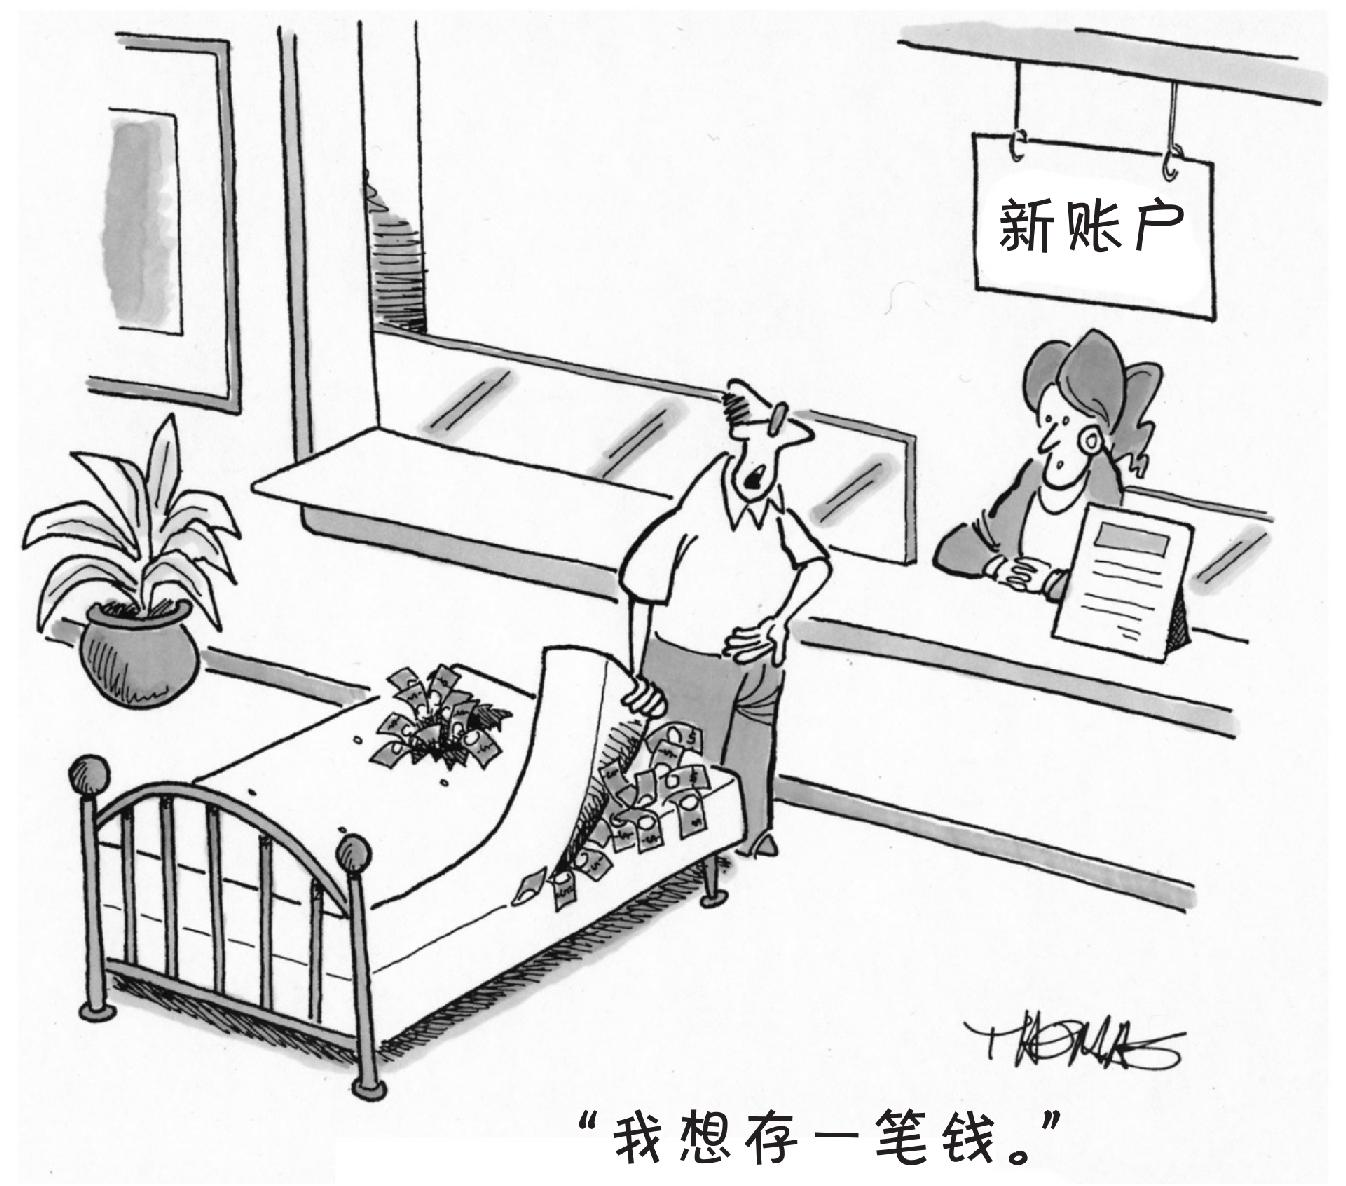
\includegraphics[width=0.68\linewidth,keepaspectratio]{image/3-2.jpg}
\caption{}\label{fig:3-2}
\end{figure}

你也许听一些财务顾问说过，这样储蓄一笔钱，就是储蓄养老金。是的，确实这就是储蓄养老金，但是我把它叫作你的赚钱机器。因为如果你往里面不断存钱，仔细维护管理好这台赚钱机器，它就会给你创造出来一大笔财富——一大笔非常安全、可靠的资产。这些投资的风险受到保障，收益税收得到减免，能够让你赚到足够多的钱，足以满足你的日常开支需要，你遇到危难时的紧急需要，以及你退休之后享受幸福晚年生活的开支需要。

这听起来很复杂吗？实际上操作非常简单。我用一个简单易懂的方式来说明一下：想象一个宝盒，你可以用储蓄来填满这个宝盒。每次领到工资收入你就往里面存钱——按照你设定好的固定比例。不管你设定的百分比是多少，你都必须一直坚持下去。不管日子是好是坏，不管发生什么情况，你都要坚持从工资收入中提取固定比例的钱存进宝盒里。为什么一定要这样坚持下去呢？因为这是复利法则的要求，哪怕你只中断了一次，复利法则都会重重地惩罚你。关于储蓄这件事，你不能这样想，我按照实际开支需要，能剩下来多少钱就存多少钱——千万不能这样随意，用这种方法来储蓄，你肯定会花得多存得少。不要让自己落到中止储蓄（甚至从储蓄里拿出钱来花）的地步，要事前做好准备，以防你连续几个月收入很少，手头钱很紧张。

每个月从工资收入里拿出来储蓄的钱，应该占多大比例对你比较合适呢？10\%还是15\%呢？没有一个标准的答案，只有一个适合你自己的答案。你的本能，你的直觉会告诉你应该是多少。你的心里觉得应该是多少呢？

那些理财专家会对你说，你应该计划至少拿出工资收入的10\%用于储蓄。不过，按照现今的经济情况来看，很多人认为拿出来15\%做储蓄要好得多，特别是你年纪超过40岁之后。（你将会在第三部分找到这样做的理由。）

\begin{BookQuote}
有谁记得那样舒舒服服而且不缺钱的好日子呢？

\hfill ——拉尔夫·瓦尔多·爱默生
\end{BookQuote}

看到这里，你可能会说：“你这些养老储蓄的建议，从道理上讲都很对。但是我手头的钱实在太紧了！少花一分钱都不行。”这样想的人并不是只有你一个。很多人都觉得他们根本负担不起一分钱的储蓄。但是坦白来说，我们要是不储蓄，后果会是根本负担不起。相信我，如果现在确实急需用钱，我们每一个人都能挤出来一些钱救急的！但要说为了我们自己的未来而攒钱，问题就来了，因为未来不是现在，它看不见，摸不着，令人感觉不真实。正是这个原因，才导致我们很难为养老定期储蓄，尽管我们知道储蓄与否会使退休生活天差地别：定期储蓄会让我们的家庭过上幸福美满的退休生活；要是不能定期储蓄，退休之后就根本没办法养活自己，只能靠政府那一点点可怜的补贴维持生存。

我们已经了解到，行为金融学家研究发现，我们在金钱方面会使用一些方式来愚弄自己做出错误的事。我会分享一些好的方法，让我们也可以用来哄骗自己去自动做正确的事。但是，这里成功的关键是，你必须让自己能够做到自动储蓄。正如伯顿·麦基尔在采访时告诉我的那样：“储蓄的最好方式是你从一开始就根本看不到钱。”这是真的，如果你根本看不到钱进来，你就会吃惊地发现，自己竟然可以找到很多方式来调整自己的开支。俗话说得好，没钱自然就不会花钱。

再过一小会儿，我就会告诉你一些自动储蓄的技巧。它们非常有效，非常容易，让你的钱甚至还没来得及进到钱包或者支票账户里，就已经改变方向直接进入储蓄账户了。首先让我们来看些真实的生活案例。他们都是只能靠工资维持生活，却能设法做到定期储蓄，持续投资，最后积累起相当大一笔财富，成就富有人生的人。

\subsection{快递小哥也能成为亿万富翁}

西奥多·约翰逊的第一份工作是快递员。1924年，他加入了刚成立的UPS（美国联合包裹服务公司），努力工作，不断升职。不过，快递员的收入有限，他的年收入从来没有超过14000美元，但是他运用了神奇的致富公式：每次领到工资，他都会拿出20\%作为储蓄，每次领到年终奖也会拿出20\%作为储蓄。他用这些钱购买UPS的股票。他心里始终有个数字，那就是自己需要从工资收入中所拿出来的用于储蓄的固定百分比——他承诺为了家庭一定要拿出来这么多钱。读到了本章的末尾，你也会愿意这样做的。

UPS股票越拆越多，加上自己继承了上一辈人的良好耐心，这些都让西奥多·约翰逊看到了自己持续不断购买的UPS股票的价值越增长越多，当他年满90岁的时候，这些股票的市值超过了7000万美元。

简直太不可思议了，你肯定会这样想。最不可思议的地方是，这个人竟然只是一个很平常的快递员，既不是像迈克·泰森那样天赋过人的运动员，也不是像弗朗西斯·福特·科波拉那样才华出众的导演，甚至不是一家公司的高管。但是西奥多·约翰逊很早就开始从工资中拿出固定比例的收入定期储蓄，投资股票，充分利用复利的巨大威力，这样做对自己的一生产生了巨大的影响，而且对无数其他人的一生产生了巨大的影响。西奥多·约翰逊还有一大家子人要养活，每个月水费、电费、煤气费好多账单必须支付，但是对于西奥多·约翰逊来说，这些账单虽然重要，但是他对自己未来的承诺更加重要——决定每月要储蓄20\%的收入就一定要把它拿出来。他总是第一个付钱来打造自己的财务自由投资基金。

到了晚年，约翰逊积累了几千万美元的巨大财富，有了这些钱，他就能够做一些非常美好和有意义的事情了。他捐赠了超过3600万美元给各种教育事业，其中包括捐赠360万美元给两家聋人学校，因为他从20世纪40年代起就几乎听不见了。他还在UPS设立了一项大学奖学金，以资助公司雇员的孩子读大学。

你听说过欧谢拉·麦库迪的故事吗？她住在密西西比州哈蒂斯堡，只有小学六年级的文化水平，是一个工作非常辛苦的洗衣女工，她整整工作了75年，天天洗衣服、熨衣服。她的生活非常简朴，花钱总是非常小心，并想方设法地从收入里省出一部分储蓄起来。“我把这些钱储蓄起来。”她这样解释自己的投资理财理念，“我绝对不会拿出来一分钱花。我总是往里面存钱。我的钱就是这样积攒起来的。”

哦，事实确实是这样的。当她87岁的时候，麦库迪的一个举动成为轰动整个美国的大新闻——这个洗衣女工捐出15万美元给南密西西比大学设立了一项奖学金。这个女人既没有银幕巨星金·贝辛格那样美丽动人的外表，也没有威利·纳尔逊那样独特的音乐天才，但是她一生都非常努力地工作，她知道自己储蓄的钱也在努力地工作。

“我想帮助其他人的孩子上大学。”她这样说。她也完全有能力这样做，当然，基础是她一生都要非常勤劳地工作，同时储蓄一大笔财富。她剩下来的一点儿钱，让自己可以小奢侈一下——给自己的房子买了一台空调。

从个人投资水平的最高层次来看，我们可以看到约翰·邓普顿爵士这个充满激情的案例。约翰爵士是有史以来最伟大的投资者之一，也是我个人的投资偶像。我非常荣幸能结识他，也采访过他几次。我把最后一次采访他的内容，也写进了“亿万富翁战术手册”那部分。下面我先简单介绍一下约翰爵士的背景，他并不是生来就是约翰爵士，他的起点其实非常低，他生在田纳西州一个普通人家里。年轻的时候他不得不从大学退学，因为他负担不起学费。但是尽管那时很年轻，他就认识到要持续不断地储蓄、投资，利用复利的神奇力量来积累财富。他承诺不管挣多少钱都要拿出来一半做储蓄，然后拿这些储蓄去投资，让这些资本用更高效的方式来工作。

约翰研究了历史，发现了一个非常清晰的模式。“托尼，你要找到非常便宜的股票，要在整个市场很悲观的时候。”他告诉我，“什么都不会让一只股票的股价下跌，除非是它卖出的压力变大。”好好想一想这句话吧。当经济形势良好，你想卖房子，会有很多人想买，你会一直等到最高出价才卖。在大牛市里，投资者想要找到价格便宜的股票很难。为什么？当经济增长、股市行情好的时候，人类的天性会让人们觉得情况将会一直持续，直到永远！但是，当突然发生灾难的时候，人们都会赶紧跑到山上避难。房子不要了，股票不要了，企业不要了。只要给钱就卖，反正不卖也不要了。正是靠着敢于在大熊市“买入”这种违反常理的举动，约翰白手起家，最后成为拥有几十亿财富的大富豪。

他是怎么做到的呢？1939年德国入侵波兰，把整个欧洲拖入了第二次世界大战，整个世界充满了恐惧和绝望。就在这个人人恐慌、疯狂抛售的时候，约翰东拼西凑了10000美元投资买入了美国纽约股票交易所里还在交易的股票。当时市场上有100只股票的交易价格跌到了1美元以下，他用这10000美元分别买了每只股票100股，其中有些公司大家都觉得很快就要破产了。但是约翰知道很多人当时忘记了的事情：夜晚不会永久，白天定会来临。金融世界的冬天只是一个季节而已，它肯定会过去，春天还会再来临的。

到了1945年，第二次世界大战结束了，美国经济飞速增长，美国股市飞速暴涨，约翰手里的股票也跟着暴涨。就这样，他从10000美元起家，投资股票，变成了身家数十亿美元的超级富翁。我们看到了同样的大牛市，从2009年3月的最低点大幅反弹，直到2013年年底，不到两年股市暴涨了142\%。但是大多数人都错过了这波大牛市。为什么？当经济下滑、股市下跌、情况变坏时，人们觉得情况会一直糟糕下去——悲观主义压倒了一切，我会在第四部分中展示给你一套方法，帮助你保持头脑清楚，继续坚定地持有，继续投资，尽管周围其他人都非常恐惧害怕，纷纷抛售股票。正是在这个非常短暂且波动很大的股市行情中，赚到那些天文数字般收益的机会才有可能出现在你眼前。

我把这些投资见解传递给我的白金合伙人，这些人加入了我创立的一个封闭性的精英小组，来支持我搞的慈善基金会，我把这些近在眼前的潜在投资机会分享给这些合伙人。比如拉斯维加斯的金沙集团，它是纽约股票交易所的上市公司。2009年3月9日，金沙集团的股价跌到了每股2.28美元。现在涨到了每股67.41美元——能够让你赚到30倍的巨大收益。

你瞧，这就是学会在别人恐惧时大胆投资的巨大威力。

那么我们能从约翰·邓普顿爵士那里学到什么？那就是如果你能够做到不让所有其他人的恐惧把你吓得思维瘫痪的话，那么你的研究、信息、行动会为你创造神奇且巨大的回报。这真是非常值得牢记的一课。我们将会在金融投资上经历更多极其艰难的日子。历史证明，这些“下跌得令人恐惧”的坏日子，就是值得大量投资以赢得投资比赛的伟大机会。

约翰知道，如果他能够每个月从自己微薄的收入中拿出一半来，他就有了投资的筹码，任何投资机会出现，他都能及时出手。但是他还有比投资更加重要的成就，约翰成了世界上贡献最大的慈善家之一。在他成为英国公民之后，英国女王为了表彰他对慈善事业做出的巨大贡献，册封他为爵士。即使在他去世之后，他的遗产也将继续捐赠：每一年，约翰·邓普顿基金会都会捐钱来奖励那些“用突破性发现推动人类进步”的人——每年约有7000万美元，比诺贝尔奖委员会十年发的奖金还要多。

西奥多·约翰逊的故事给你最大的启发是什么？你不需要成为一个投资天才，也能获得财务自由。

听了欧谢拉·麦库迪的人生传奇又给你什么启发呢？即使一个天天凭力气干活的洗衣女工，也可以把小钱积累成很大一笔钱，让自己的人生过得很有意义。

这三个聪明智慧的投资者会给你什么样的启发教育呢？承诺遵守一个非常简单却十分坚定的储蓄原则，每一次拿到工资收入，先从中拿出来一部分储蓄，这就是你首先付给自己追求未来梦想的投资基金，利用复利的巨大力量让你的储蓄投资不断升值，让你的人生达到你梦想都不能企及的高度。

\begin{BookQuote}
最困难的事是下决心行动，之后的事只要坚持就行了。

\hfill ——阿梅莉亚·埃尔哈特
\end{BookQuote}

那么你打算从工资收入中拿出来储蓄投资的钱应该占多大的百分比呢？西奥多·约翰逊拿出的是20\%，约翰·邓普顿拿出的是50\%。对于欧谢拉·麦库迪来说，很简单却很有智慧，就是有一分钱就存一分钱：把每一分钱都存到一个能够产生利息的储蓄账户，不断存钱，不断利滚利，不断增长。

那么你呢？你脑子里是不是有了从收入里拿出来储蓄的百分比数字了呢？太棒了！现在就做出决定，做出承诺，现在就开始迈出你追求财务自由的简单7步投资法的第一步吧！现在就做出你一生最重要的财务决策吧！现在就决定成为一名投资者，而不只是一名消费者吧。要做到这些，你只需要决定从工资收入中拿出一部分钱，坚决不花，用它来做储蓄和投资，这些钱只是为了你和你的家庭创建更加美好的未来，而不为其他任何人。

我再重复一次，一切只是为了你，为了你的家庭，为了你的将来。这些钱坚决不能花，不能用储蓄的钱去GAP（盖璞）或者Kate Spade（凯特·丝蓓）专卖店买衣服，也不能用储蓄的钱去那些昂贵的餐馆吃饭，更不能用储蓄的钱去买新车替换掉那辆还能再跑50000英里的旧车。不要只想这些储蓄今天给你带来的损失，而要专注去想这些储蓄明天会给你创造出多么巨大的收益。为了储蓄更多，以后不要再出去跟朋友吃饭，出去吃一顿晚饭，很浪费钱，比如要花50美元外出就餐，为什么不订一个两人份的比萨，再来几瓶啤酒，然后和你的朋友们AA制分摊餐费呢？这样一个人只需要花10美元。和出去大吃一顿花掉50美元相比，每顿饭能省下40美元，每次都让你在投资理财这个游戏上又领先了一小步。

才省40美元，有必要吗？40美元算啥呀？是的，你是对的，一个星期才出去吃一次，只能省40美元，是没有多少钱。但是如果每个星期都能省下40美元，然后用这些钱去投资，经过很多年后，到你退休时，它就能升值成很大一笔钱。你可以自己算一算：每个星期节省40美元，一年52个星期，你就能节省出来2000多美元。现在你知道复利的力量了，用这2000多美元去投资，复利的巨大力量就能让你多年之后实现很大一笔收益。收益到底有多大呢？难道会有50万美元吗？是的，100万美元的一半！那如果你有本杰明·富兰克林那样的投资顾问，他们会告诉你把这些钱投到股市里，如果未来40年你能每年获得8\%的复利收益率，那么你每周节省的40美元（每年节省的2080美元），最后创造出来的财富会有581940美元！有了这么多钱，你可以订比萨时再多订一块儿——想买什么都能买得起。

你开始明白如何利用复利的巨大力量为你创造财富了吗？只需要几个小小的持续行动就行了。如果你每个星期能省的钱远远超过40美元，那么你赚的钱不就更多了吗？即使每周只能节省100美元，这也意味着未来你在最急需用钱的时候，你的养老金里会有100万美元。这个差别巨大。

记住，你根本不能开始发挥复利的巨大威力，除非你承诺每次拿到收入就留出一部分来储蓄——这是最重要的事。毕竟，你有钱才能做投资人，没有钱永远也成不了投资人！储蓄是投资的前提，是投资的基础：储蓄的资本是创造财富的基础，没有储蓄就不能投资，没有储蓄就说明你只是一个靠工资挣钱的人；定期储蓄、持续投资让你成为一个能靠投资挣钱的投资者。所有财富、所有投资都开始于储蓄，你把自己收入的一部分拿出来自动存起来，去做投资，只用于自己和自己家庭的未来。

从你的工资收入中拿出来储蓄的钱占多大比例合适呢？10\%？12\%？15\%？20\%？

找个你自己能够储蓄的最大比例，并圈起来。

用荧光笔涂上。

在上面敲几下。

承诺做到。

实际做到。

自动做到。

如何自动做到拿出工资收入的固定比例进行储蓄呢？你可以从本书的官方网站上下载一个免费的App。这是一个开启你投资理财之旅的极好方法，利用这个程序，你可以设定自动提醒，以确保能够实现你的投资理财新计划。如果你还没有这样做，现在马上去做吧！这个手机应用程序会指导你走好以下几个简单的投资理财步骤：

\begin{itemize}
\item 如果你有固定工资，你最有可能制订一个自动储蓄计划。你只需要打个电话给人力资源部，让他们把你工资收入的一个具体比例（完全由你决定的比例）直接打到你的退休金账户里。
\item 如果你已经有了一个自动工资扣款计划，钱直接打到你的401(k)退休金账户里，你可以提高扣款比例。（在本书接下来的部分，我将会向你展示，如何确保你的退休养老储蓄计划能够按照合理有效的方式设计，让你确实可以“赢得”这场投资游戏比赛，确定你没有支付隐性费用，能让你的钱自由自在地在复利的环境中增长。理想的情况是能够延迟纳税，甚至完全免税，让你的财富增长最大化。
\item 但是如果你是自由职业者，或者你拥有自己的企业，或者是做代理按业绩提成的，你该怎么办呢？没问题。只要设立一个从你的支票账户向退休金账户自动转账的计划就行了。
\end{itemize}

明白你要做什么了吗？太棒了！

你如果根本没有退休金账户，那又该怎么办呢？那你就没有地方来存放你指定的储蓄资金了。很简单，现在就停下来马上上网，找一家银行或者金融机构，开个储蓄账户或者退休金账户就行了。互联网上有好多选择，能帮你确定哪家金融机构更加适合你。你也可以在我们提供的App里面找一个合适的开户银行。如果你不喜欢网络科技，想自己亲自动手，你可以直接走到大街上，到银行开个储蓄账户或者退休金账户。

最好什么时候开始做这件事呢？现在不正是最好的时候吗？

开始，我等着你……

\begin{BookQuote}
你如果不愿意工作，就不得不先去工作挣到足够的钱，好让你再也不会不得不去工作。

\hfill ——奥格登·纳什
\end{BookQuote}

好极了，你回来了。你搞定了储蓄这件事了。祝贺你！你刚刚做出了你人生最重要的财务决策——通向财务自由的简单7步投资法的第一步。现在你已经走上正路了，去把你的梦想变成现实吧。

在后面的内容里，我会和你分享一些最安全而且最有确定性的投资策略，让你的钱不断增值，而且是用一种税收优惠的方式！但是现在让我们先来确定你的工资收入用于储蓄的比例吧，因为你只有有能力做到有系统、有计划地持续储蓄，才能在此基础上创造出你未来的财务自由。大多数人可能都知道这一点，起码在某种程度上知道，但是你如果还是什么事也没有做，那么你其实并不知道这一点。传统的说法是知识就是力量，这完全不对，知识不是力量，知识只是潜在的力量。知识并不代表掌握，实干才是掌握。实干总是会压倒知识的。

\begin{BookQuote}
我痛恨输，甚至胜过我想赢。

\hfill ——比利·比恩（电影《点球成金》中由布拉德·皮特扮演的棒球俱乐部总经理）
\end{BookQuote}

你已经学到所有该学的东西了，可是你还没有迈出第一步，把自己工资收入的一定比例拿出来，储蓄起来赚取复利，以不断增值，那该怎么办呢？有什么事情在阻碍你吗？到底出了什么事情呢？你不能有组织、有计划地定期储蓄，是不是因为你觉得拿出来储蓄的这些钱好像是一种牺牲、一种奉献、一种损失，而不是一个礼物——今天的你送给未来的一个礼物呢？在寻找答案的过程中，我遇见了什洛莫·贝纳茨，他是加利福尼亚州大学洛杉矶分校安德森管理学院的教授。他说：“托尼，问题是人们总觉得未来是不真实的，所以为了未来做储蓄很难。”贝纳茨和理查德·塞勒一起合作搞研究，理查德·塞勒获得过诺贝尔经济学奖，是芝加哥大学的教授。他们两人想出来一个超级有效的解决办法，叫作“明天储蓄更多”（SMarT），其前提非常简单，但非常有力：你如果现在觉得储蓄更多钱让你很受伤、很痛苦的话，那就等到下一次涨工资再储蓄更多。

他们俩是怎么想到这个办法的呢？首先，什洛莫告诉我，他们必须应对人类喜欢马上得到满足的挑战，科学家称之为“即时偏见”。他给我举了一个例子：有一次他问一群学生，再过两周他们再见面时，他们想要得到一根香蕉还是几块巧克力当零食吃呢？75\%的人都说想要香蕉。但是过了两周之后，当这两种东西摆在他们面前时，80\%的人都拿了巧克力！“自我控制在未来并不是问题。”什洛莫说。储蓄也是同样的道理。他告诉我：“我们知道我们应该储蓄。我们知道我们明年会储蓄。但是现在我们要出去把钱花掉。”

我们人类这个物种，天性如此，不但偏爱今天胜过明天，而且我们非常痛恨我们正在失去某种东西的感觉。为了说明这一点，什洛莫给我讲了一个研究实验，这个实验是用猴子这个我们不太远的“亲戚”来做的。科学家给一群猴子发了一个苹果，与此同时测量猴子的生理反应。这些猴子非常激动！然后，科学家给了另外一群猴子两个苹果。它们的生理反应也是非常激动。再做一个变化：原来给两个苹果的猴子，现在从它们手里拿走一个苹果，它们手里还剩一个苹果。你猜结果发生了什么样的事情呢？你猜对了，它们非常生气，简直气炸了。（科学地说）你想想，要是这种事发生在你身上，你是不是也非常生气呢？事实上这种事情不就经常发生在我们每个人身上吗？我们忘了自己已经拥有的，是不是？请记住这个实验，等到下一章，我给你讲亿万富翁阿道夫·默克尔的故事时，它会让你豁然开朗。

最核心的观点是，如果我们觉得自己正在失去某些东西，我们就会极力避免，因为我们不愿意失去。正是因为这个原因，很多人不储蓄不投资。储蓄听起来好像你放弃了某些东西，你今天失去了某些东西。但是其实你没有，储蓄是今天的你给自己的一份礼物，可以让自己得到大脑的平静，内心的安定，还有未来的一大笔财富。

那么什洛莫和塞勒是怎么来应对这些挑战的呢？他们想出来一套简单的做法，让你感觉储蓄毫无痛苦。这种做法完全符合人的天性。正如什洛莫在TED演讲中所说的，“明天储蓄更多的计划鼓励员工下一年储蓄更多的钱，来实现自己未来的梦想——到了未来某个时候，我们可以想象自己正在吃香蕉，正在社区做义工，做更多的体育锻炼，做所有正确的事情。”

明天储蓄更多这个计划是这样做的：你同意自动储蓄接下来你工资收入的一小部分，比如10\%或者5\%，甚至只有3\%（这个储蓄比例简直太低了，你甚至根本觉察不到有没有这一点钱的差别）。接下来，你承诺未来会储蓄更多，但是只在你工资收入增加时才会提高储蓄比例。每一次你的工资增加的时候，工资收入拿出来用于储蓄的比例会自动增加一点，但是你根本不会感觉到这是一种损失，因为你一开始承诺未来储蓄更多时，还根本看不到未来增加的工资收入。

什洛莫和塞勒两个教授第一次试验这个明天储蓄更多的计划，是在20多年前，在美国中西部的一家公司里，那里的蓝领工人一听说要做这样的实验就说，他们的工资很低，根本不够花，挤不出一分钱去做储蓄。这些研究者费了很大力气才说服他们，让公司可以自动地从他们的工资里扣除3\%，储蓄到他们的退休金账户里。以后每一次他们加薪的时候，工资用于储蓄的比例再增加3\%。结果如何呢？简直令人震惊！仅仅过了五年，只有三次加薪，这些工人原来以为自己根本拿不出1美元去储蓄，结果他们的储蓄比例高到接近14\%！其中65\%的工人实际上的平均储蓄比例高达19\%。

当储蓄比例达到了19\%时，你就接近西奥多·约翰逊的储蓄比例了。要知道，这个UPS的快递员正是坚持每次领到工资就储蓄20\%去购买UPS的股票，结果创造出7000万美元的巨大财富的。明天储蓄更多的计划，一点儿痛苦也没有，而且确实有效。一次又一次的实验证明这个计划非常有效。

我来给你看张图，什洛莫教授用这张图来描述员工一次次提高工资收入的储蓄比例，会对这个员工的生活产生什么样的影响。

\begin{figure}[htbp]
\centering
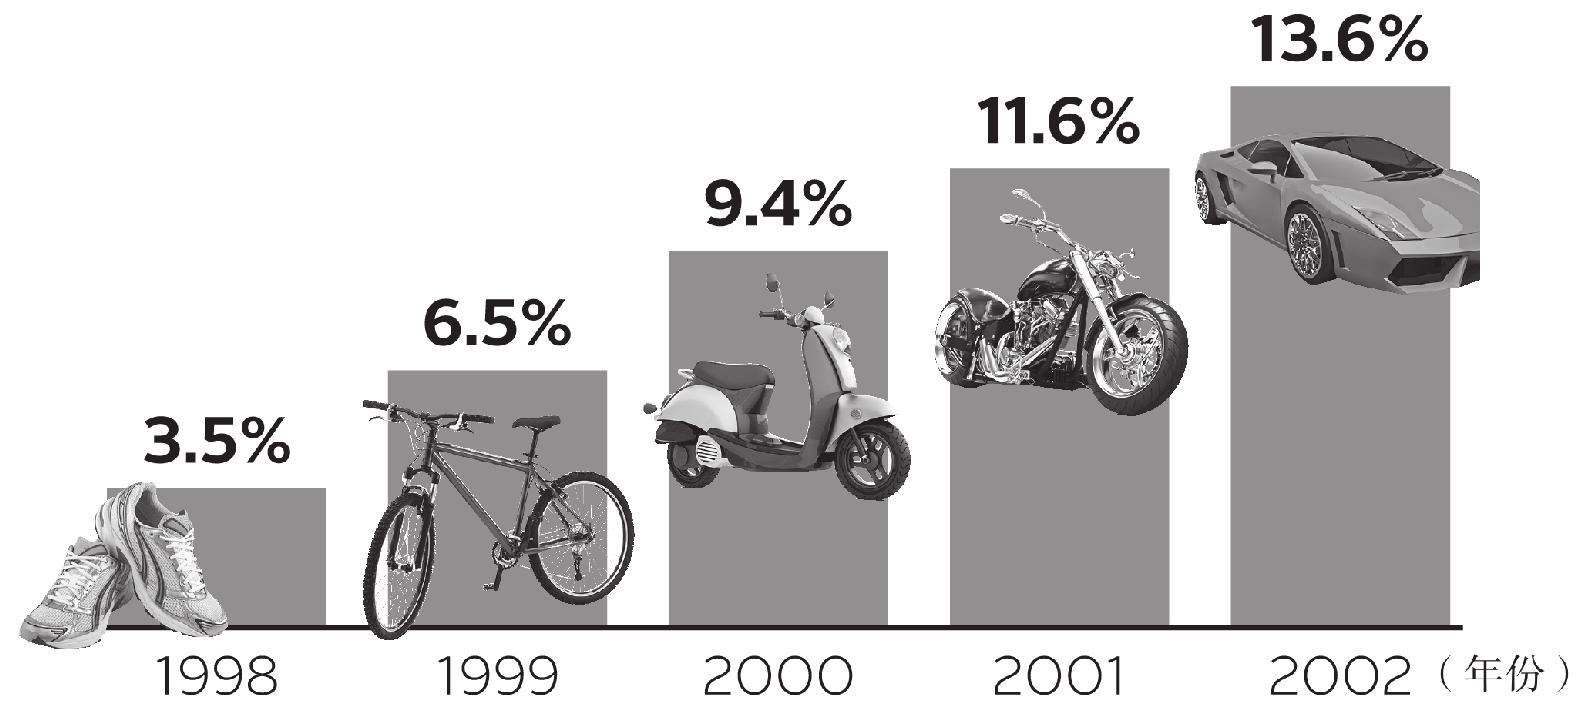
\includegraphics[width=0.88\linewidth,keepaspectratio]{image/3-3.jpg}
\caption{}\label{fig:3-3}
\end{figure}

当工资收入的储蓄比例是3\%的时候，图中出现的是一双球鞋的图片——因为你储蓄起来的工资收入的3.5\%，未来增值的空间有限，只够买双球鞋。工资收入的储蓄比例是6.5\%的时候，你未来赚的钱就够买辆自行车了。工资收入的储蓄比例约14\%的时候，未来赚的钱就可以买辆豪华小汽车了。很明显，开着豪华小汽车的晚年生活，要比只能穿着球鞋自己走路强多了。3.5\%和14\%的储蓄比例，会让你的晚年生活像穿球鞋和开豪车一样大。

现在规模比较大的企业有60\%都提供类似于明天储蓄更多的计划。去了解一下你的公司是否提供这样的计划，如果没有，拿着这本书给公司的人力资源部看一看，问问公司能不能给你设置类似的储蓄计划。

当然，你还需要好好干活，真正“挣到”你的加薪——你的老板不会因为你很有礼貌地请求加薪，就给你加薪的。但是一旦你加薪了，你就完全可以自由决定是拿出所有的加薪或者只是一部分来增加储蓄，这取决于你的个人情况。在某些情形下，如果你的公司能够匹配你的个人能力，老板会帮你做到储蓄加倍——你的财富积累之路就快多了。

如果你的老板并不提供这种计划，你可以自己创立一个。你可以从储蓄5\%的工资收入开始（不过我鼓励你如果经济条件允许的话，一开始的储蓄比例至少不低于10\%）。一发工资，这5\%的钱就自动进入你的财务自由投资基金，然后再承诺每一次加薪就把你的储蓄比例提高3\%。上网或者打电话，就可以实际启动你的明天储蓄更多的计划，让计划变成现实。今天你就能做到，锁定你的未来，用最没有痛苦的方式。你根本找不到借口不去这样做。你甚至可以用我们的手机App，我们给你预先写好了电子邮件，你可以马上发给你的老板或者人力资源部的负责人，这样你就可以立刻启动这套流程了。是不是非常容易呢？马上去做，现在！

但是你如果是自由职业者，该怎么办呢？如果你有自己的企业，你觉得你需要把每一分钱都投入到企业里，该怎么办呢？相信我，你会找到办法的。如果现在有一种新的税收推出来了，你必须给政府多交纳10\%的税，甚至是多交纳15\%的税，你会怎么办呢？你肯定恨死它了！你会高声尖叫，这简直是谋杀！但是没办法，你还是会想办法交纳这笔税的。所以你可以这样想，把你从工资收入里拿出来储蓄的这笔钱看作一种税，你“必须要付”的税。这些钱不是交到政府手里的，而是要交给你的家庭和未来的你的！或者想象你自己就是一个卖东西的零售商，你必须第一个付款给这个零售商。如果这是必须做的事情，你就会做到。但是在这种情况下，这笔钱是你和你的家庭的东西，将会永远保存下去，对不对？这就是积累财富的所有秘密：挣钱更多，花钱更少，自动储蓄。

\subsection{天空中火一般燃烧的文字}

年轻的时候，我偶然读到了乔治·萨缪尔·克拉森1926年的经典著作《巴比伦最富有的人》。那本书用古老的寓言故事讲了一个像常识一样的投资理财建议。我建议所有人都要好好地读读这本书。多年以来，有段话一直印在我脑海里：“你挣的所有钱里面有一部分必须被保存起来。”早上醒来就对自己说一遍这句话，每天中午对自己说一遍这句话，每天晚上对自己说一遍这句话，每天每过一个小时对自己说一遍这句话。不停地对自己说这句话，直到这句话的文字就像天空中的火焰一样，深深地印在你的脑海里。深刻理解这句话的意思。满脑子都是这个想法。从你的收入中拿出一定的比例，你觉得比例合适就行，不要少于10\%。然后把钱储蓄起来。如果需要的话，仔细安排好你的其他生活开支，好让自己储蓄的钱能达到想要的比例。不管如何花钱，首先把这部分钱拿出来做储蓄，一分钱也不能花。

\begin{BookQuote}
只有乐善好施的意图不行，那样就没有人会记得“好撒马利亚人”。他还得有钱。

\hfill ——玛格丽特·撒切尔
\end{BookQuote}

先把那部分钱储蓄起来，我的朋友，记住。然后按照这个原则行动，你储蓄的那部分钱占你收入多大比例并不重要，重要的是开始储蓄。在理想的情况下，你从收入里拿出来储蓄的比例不要低于10\%。但是，随着时间推移，不断提高你的储蓄比例，使其达到相当高的程度。

\subsection{下一步}

现在你已经设定了一个自动投资计划——你的财务自由投资基金，你新的赚钱机器。也许现在会有两个问题出现在你的脑海里：第一，我把这些钱放到哪里呢？第二，我需要积累多少钱才能得到财务安全和财务自由呢？我们下面会清楚地回答这两个问题，让你一听就明白。答案来自全世界投资理财做得最成功的人士。

但是，首先我们需要了解你投资的真正目的是什么。你个人对财务自由的渴望背后的更深层次的愿望是什么呢？财富对于你来说真正的意义是什么呢？你真正追求的是什么呢？我们来快速浏览一下，只有几页纸，看看你如何能够掌控金钱。
